\ylDisplay{Jõulukaunistus} % Ülesande nimi
{Valter Kiisk} % Autor
{lõppvoor} % Voor
{2010} % Aasta
{G 8} % Ülesande nr.
{8} % Raskustase
{
% Teema: Elektriahelad
\ifStatement
Jõulukaunistuse hankimiseks majandussurutise tingimustes otsustas Juku
ühendada jadamisi kokku 50 valgusdioodi ja toita seda ahelat läbi alaldusdioodi $D$ otse
võrgupingega (vt joonist). Voolu piiramiseks on ahelasse lülitatud takisti
ning voolu pulsatsiooni väljasilumiseks kondensaator. Pinge alaldusdioodil on
tühine, igal valgusdioodil aga $U_d=\SI{3}{V}$. Kui suure takistusega $R$ ja maksimumvõimsusega $N$ tuleks valida
takisti, kui valgusdioodid taluvad voolu kuni $I=\SI{20}{mA}$? Kui suure mahtuvusega $C$
kondensaator kindlustab, et voolutugevuse pulsatsioon jääb $\alpha=\num{5}\%$ piiresse? Võrgupinge
sagedus on $f=\SI{50}{Hz}$ ning amplituudväärtus $U_0=\SI{311}{V}$.

\begin{center}
	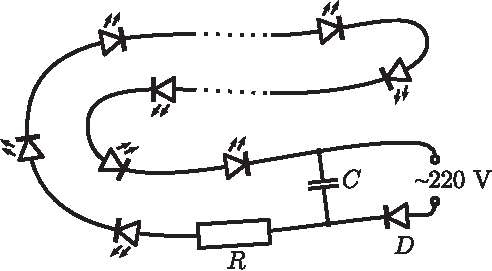
\includegraphics[scale=0.75]{2010-v3g-08-elektrikuunlad2}
\end{center}
\fi


\ifHint
Nominaalses töörežiimis on iga valgusdioodi pinge $U_d$ ja vool maksimaalselt \SI{20}{mA}. Teades võrgupinge maksimaalset pinget on võimalik leida takisti takistus ja maksimumvõimsus. Ühe täisperioodi jooksul tuleb pingelanguse muut kondensaatoril takisti arvelt. Seejuures on kondensaatori plaatide laengumuut leitav täisperioodi pikkusest ja ahela voolutugevusest.
\fi


\ifSolution
Maksimaalne pinge, milleni kondensaator laadub, võrdub võrgupinge
amplituudväärtusega \SI{311}{V}. Sellest takistile langeb pinge
$\SI{311}{V}-\num{50}\times\SI{3}{V}=\SI{161}{V}$. Seega takistuse väärtus peab olema
$\SI{161}{V}/\SI{20}{mA}\approx\SI{8}{k\ohm}$ ja sellel eraldub võimsus
$\SI{161}{V}\times\SI{20}{mA}\approx\SI{3.2}{W}$. Peale pinge amplituudväärtuse
saavutamist peab kondensaator olema suuteline vahelduvvoolu ühe perioodi (\SI{20}{ms})
jooksul valgusdioodide ahelat toitma nii, et pingelang takistil (ja seega ka
kondensaatoril endal) kukub mitte rohkem kui $\num{0.05}\times\SI{161}{V}=\SI{8}{V}$
võrra. Samas kondensaatorilt võetakse sama aja jooksul elektrilaeng
$\SI{20}{mA}\times\SI{20}{ms}=\SI{0.0004}{C}$. Seega nõutav mahtuvus on
$\SI{0.0004}{C}/\SI{8}{V}=\SI{50}{\micro F}$.
\fi
}